\section{Quelques captures d'écran}
\begin{figure}[h]
	\center
	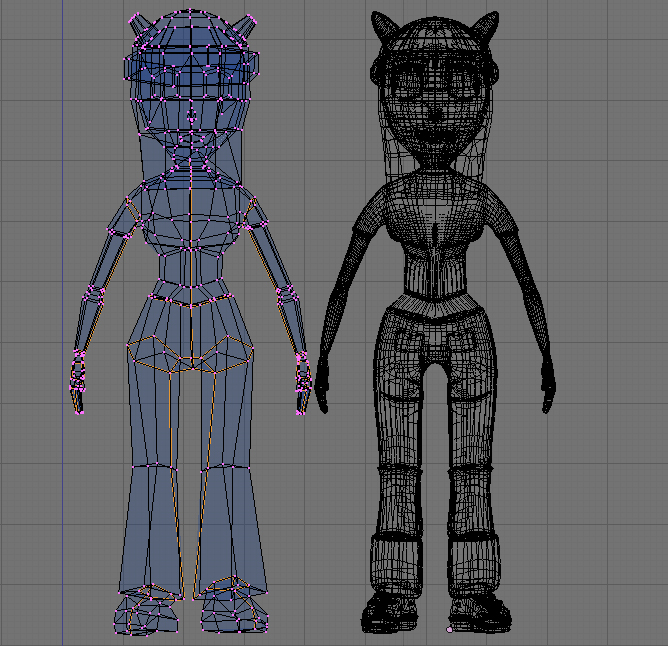
\includegraphics[scale=0.4]{visuel/mesh.jpg}
	\caption{Visualisation des meshes}
\end{figure}

\begin{figure}[!h]
	\center
	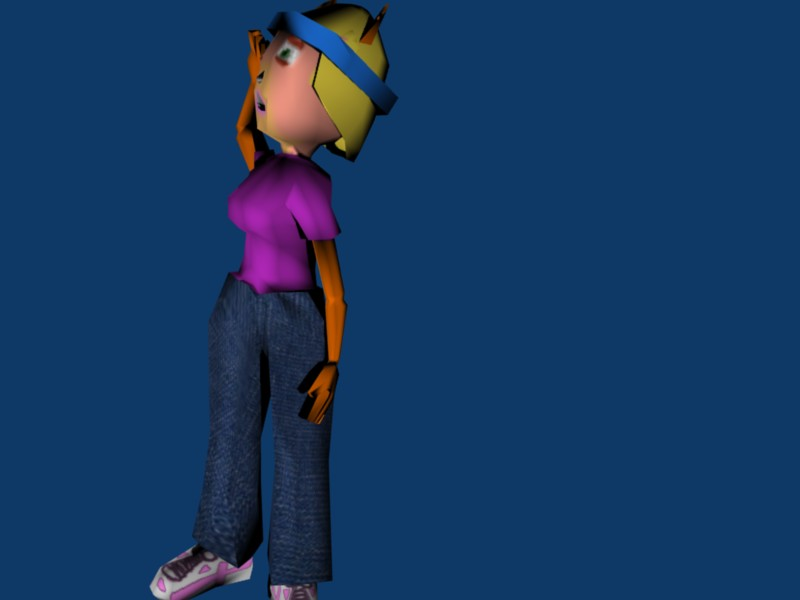
\includegraphics[scale=0.4]{visuel/rendu_test1.jpg}
	\caption{Test de rendu d'un personnage}
\end{figure}

\begin{figure}[!h]
	\center
	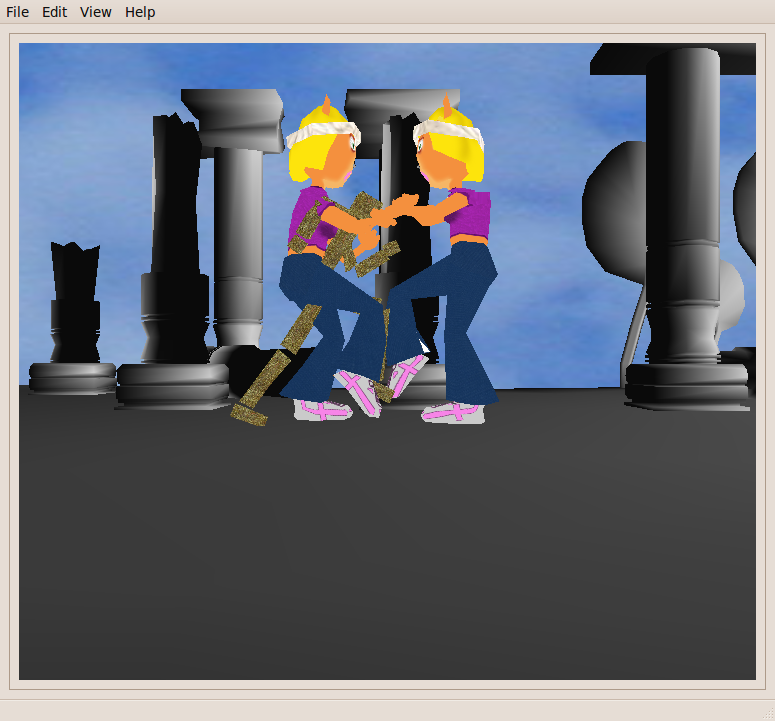
\includegraphics[scale=0.4]{visuel/capture-rev140-1.png}
	\caption{Vue globale de l'arène}
\end{figure}

\newpage
\section{Pseudo-code de l'IA}

\begin{scriptsize}
\begin{verbatim}
Toutes les x frames : regarde s'il change de comportement (modulé par le comportement)


actions possibles :

direction droite
direction gauche
sauter
coup1
coup2
projectile
bloquer

_______________________________________________________________

structures de données :

arbre attaque
arbre defense
barette mémoire (file) "enchainement player" (même nb de barettes que de joueur)  
barette mémoire (file) "enchainement bot"
barette action (file)

recupération d'un argument de main pour le profil du joueur
stockage des arbres de probabilités dans les fichiers textes

_______________________________________________________________

RECUPERATION DU RADAR + ACCES A LA MEMOIRE

qui est mon ennemi ?
  * y a-t-il plus d'un ennemi ?
    -> si non : 
      * le choix est fait
    -> si oui : 
      * choix entre différentes propositions
      -> quel est mon caractère ? (agressif, peureux, vengeur, etc...)
      /*
      Critères de selection
      si ennemi est très très bas en PV alors l'option correspondante recevra un bonus enorme
      si un ennemi a infligé + de 50 % de dégâts (pourcentage modulé par le caractère) alors il cherche a se venger
      si un ennemi a reçu + de 50 % de dégâts (idem) alors il va chercher à l'achever
      si les probabilités sont proches entre elles alors l'option "plus près" 
      */
	
        -> le plus près
        -> le plus mal en point
        -> celui qui a infligé le plus de dégât
        -> celui qui a été le plus tapé

remplit la mémoire sur l'action précédente
  * quelle a été l'action du player ?
    * si la barette contient X (un seuil pédéfini) actions alors reset de la barette
    * si la dernière entrée de la barette date d'au moins X frame alors reset de la barette
    * enregistrement de l'action dans une barette mémoire temporaire "enchainement player"
  * le bot a-t-il fait des dommages ?
    -> si non : 
      * si la barette contient X (un seuil pédéfini) actions alors reset de la barette
      * si la dernière entrée de la barette date d'au moins X frame alors reset de la barette 
      * enregistrement de l'action précédente dans une barette mémoire temporaire "enchainement bot"
    -> si oui :
      * mise à jour du graphe d'attaque en parcourant selon l'enchainement effectué
  * le bot a-t-il encaisser des dommages ?
    -> si oui :
      * récupération de la barette temporaire "enchainement player"
      * mise à jour du graphe de defense en parcourant selon l'enchainement effectué (malus)
    -> si non :
      * récupération de la barette temporaire "enchainement player"
      * la dernière entrée de la barette date de moins X frame (obsolète)
        -> si oui : 
          * reset de la barette
        -> si non :
          * mise à jour du graphe de defense en parcourant selon l'enchainement effectué (bonus)   
			
quel est mon état ? choix :
  -> quel est mon caractère ? (agressif, peureux, vengeur, etc...)
	
  /*
  Notes comportement
  Certains possèdent des conditions ("instructions prioritaires")
  Exemple : agressif ne doit pas laisser de repos à son adversaire 
  (pas attendre avant d'attaquer) et doit se trouver à middle range de sa cible
  */
	
    -> attaque
    -> défense
		
ai-je suffisamment de probabilités pour cet ennemi ? 
// seuil fixé dans les arbres de proba et modulé par le caractère
  -> si non : 
    * comportement passe à "recherche information"
    // c'est-à-dire remplir l'arbre de probabilité correspondant)
		
    /*
    Notes "recherche information"
    Parcours de l'arbre correspondant.
    Si une inconnue est rencontré sa priorité devient maximale,
    si plusieurs inconnues existent alors choix aleatoire. 
    */
		
    -> si oui : 
      * alors parcours de l'arbre de probabilité correspondant
        -> comportement X

mise à jour de la barette d'action
  * remplir la barette avec les actions données par la comportement
    -> y a-t-il un événement majeur ?
    // apparition super bonus, point de vie proche de zéro, se maintenir à middle range
      -> si oui :
        * insérer cette action en tête de barette stratégie
			
  * vérifié la validité de l'action (si elle n'a pas déjà été faite)		
  * lancer la première action de la barette
\end{verbatim}
\end{scriptsize}
